\clearpage
\subsection{Getting started with MOSL}
\texHeader
\hypertarget{static:starting tex}{}

\begin{itemize}

\item[$\blacktriangleright$] \hypertarget{static tex}{Begin a} new metamodel project from eclipse by navigating to the \texttt{New Metamodel} button on the
toolbar. In the dialog that appears, enter `LeitnersLearningBox' as the project name, and select \texttt{Textual (MOSL)}  (Fig.~\ref{fig:new_project}).

\begin{figure}[htbp]
	\centering
  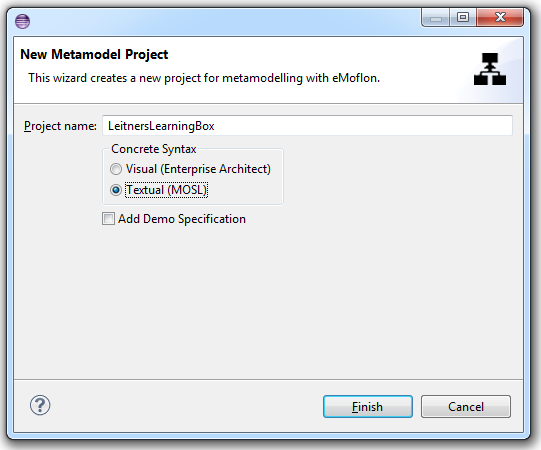
\includegraphics[width=0.7\textwidth]{eclipse_newMetamodelTextPlain}
	\caption{Create a new metamodeling project}
	\label{fig:new_project}
\end{figure}

\item[$\blacktriangleright$] Expand the project as deep as it goes. Your Package explorer may look different than ours (Fig.~\ref{fig:expanded_folders}),
depending on whether or not you completed the Demo in Part I. In an effort to keep things clear as possible, we have removed them from our workspaces, but
still recommend keeping them for future reference.

\begin{figure}[htbp]
	\centering
  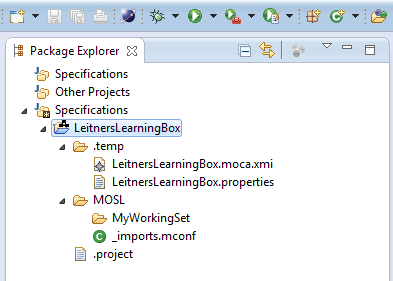
\includegraphics[width=0.5\textwidth]{eclipse_foldersExpanded}
	\caption{Expanded project files}
	\label{fig:expanded_folders}
\end{figure} 

\clearpage

\item[$\blacktriangleright$] You should be able to see two folders, \texttt{.temp}, and \texttt{MOSL}, and one subfolder, \texttt{MyWorkingSet}\footnote{if you
can't, make sure your `Top Level Elements' are set to \texttt{Working Sets}.}. We're most insterested in \texttt{MyWorkingSet}, which will store the collection
of files and \emph{unifies} the things we need for our Leitner's Box\footnote{for detailed review on the explorer structure, review Part I.}.

\vspace{0.5cm}

\item[$\blacktriangleright$] Right click on your current workspace folder, \texttt{MyWorkingSet}, and create a new subfolder. Name it
`LearningBoxLanguage'. This is now the container for all your modelling files. In essence, this is the location all your generated
files will be derived from.

\vspace{0.5cm}

\begin{figure}[htbp]
	\centering
  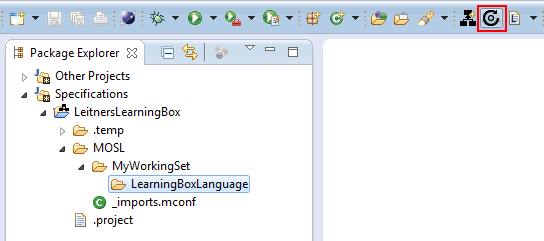
\includegraphics[width=0.8\textwidth]{eclipse_preBuild}
	\caption{}
	\label{fig:all_files}
\end{figure} 

\vspace{0.5cm}

\item[$\blacktriangleright$] To finalize initalization of your metamodel, navigate to ``Build (Without cleaning),'' found beside ``New Metamodel'' on the
toolbar (Fig.~\ref{fig:all_files}).

\item[$\blacktriangleright$] Navigate to ``LearningBoxLanguage/model.'' There, you'll be able to see a \texttt{LearningBoxLanguage.ecore} file. This is the
concrete model for your metamodel, which will adhere to any types and contraints you define within
``LeitnersLearningBox/MOSL/MyWorkingSet/LearningBoxLanguage.''

\item[$\blacktriangleright$] You've just finished creation process of a new metamodel project! If you would like to review specific details on the textual 
project structure, read Section 4.2 in Part I\footnote{\downLink}.

\fancyfoot[R]{$\triangleright$ \hyperlink{static:classes tex}{Next}}

\end{itemize}
